%!TEX program = pdflatex 
\documentclass[french, 10pt]{article}

\widowpenalty=10000
\clubpenalty=10000
\hyphenpenalty=5000
\tolerance = 10000


%% Langue et compilation

\usepackage[utf8]{inputenc}
\usepackage[T1]{fontenc}
\usepackage[french]{babel}
\usepackage{caption}
\usepackage{subcaption}
%% LISTE DES PACKAGES

\usepackage{mathtools}     % package de base pour les maths
\usepackage{amsmath}       % mathematical type-setting
\usepackage{amssymb}       % symbols speciaux pour les maths
\usepackage{textcomp}      % symboles speciaux pour el text
\usepackage{gensymb}       % commandes generiques \degree etc...
\usepackage{tikz}          % package graphique
\usepackage{wrapfig}       % pour entourer a cote d'une figure
\usepackage{color}         % package des couleurs
\usepackage{xcolor}        % autre package pour les couleurs
\usepackage{tcolorbox}     % package pour faire de jolis cadres
\usepackage{pgfplots}      % pacakge pour creer des graph
\usepackage{epsfig}        % permet d'inclure des graph en .eps
\usepackage{graphicx}      % arguments dans includegraphics
\usepackage{pdfpages}      % permet d'insérer des pages pdf dans le document
%\usepackage{subfig}        % permet de creer des sous-figure
\usepackage{pst-all}       % utile pour certaines figures en pstricks
\usepackage{lipsum}        % package qui permet de faire des essais
\usepackage{array}         % permet de faire des tableaux
\usepackage{multicol}      % plusieurs colonnes sur une page
\usepackage{enumitem}      % pro­vides user con­trol: enumerate, itemize and description
\usepackage{hyperref}      % permet de creer des hyperliens dans le document
\usepackage{lscape}        % permet de mettre une page en mode paysage
\usepackage{lmodern}       % permet d'avoir certains "fonts" de bonen qualite
\usepackage{fancyhdr}      % Permet de mettre des informations en hau et en bas de page      
\usepackage[framemethod=tikz]{mdframed} % breakable frames and coloured boxes
\usepackage[top=1.5cm, bottom=1.5cm, left=2.5cm, right=2.5cm]{geometry} % donne les marges
\usepackage[font=normalsize, labelfont=bf,labelsep=endash, figurename=Fig.]{caption} % permet de changer les legendes des figures
\usepackage{time}

%% LIBRAIRIES

\usetikzlibrary{plotmarks} % librairie pour les graphes
\usetikzlibrary{patterns}  % necessaire pour certaines choses predefinies sur tikz
\usetikzlibrary{shadows}   % ombres des encadres
\usetikzlibrary{backgrounds} % arriere plan des encadres


%% MISE EN PAGE

\pagestyle{fancy}     % Défini le style de la page

\renewcommand{\headrulewidth}{1pt}      % largeur du trait en haut de la page
\fancyhead[L]{Dossier de recherche}         % info coin haut gauche
\fancyhead[R]{Agrégation externe spéciale de Physique-Chimie: option Physique}  % info coin haut droit

% bas de la page
\renewcommand{\footrulewidth}{1pt}      % largeur du trait en bas de la page
\fancyfoot[L]{Gabriel \bsc{LE DOUDIC}}  % info coin bas gauche
%\fancyfoot[R]{compilé le \today~ à \now }%Préparation de l'Université de Rennes 1}                         % info coin bas droit


\setlength{\columnseprule}{1pt} 
\setlength{\columnsep}{30pt}



%% NOUVELLES COMMANDES 

\DeclareMathOperator{\e}{e} % permet d'ecrire l'exponentielle usuellement


\newcommand{\gap}{\vspace{0.15cm}}   % defini une commande pour sauter des lignes
\renewcommand{\vec}{\overrightarrow} % permet d'avoir une fleche qui recouvre tout le vecteur
\newcommand{\bi}{\begin{itemize}}    % begin itemize
\newcommand{\ei}{\end{itemize}}      % end itemize
\newcommand{\bc}{\begin{center}}     % begin center
\newcommand{\ec}{\end{center}}       % end center
\newcommand\opacity{1}               % opacity 
\pgfsetfillopacity{\opacity}

\newcommand*\Laplace{\mathop{}\!\mathbin\bigtriangleup} % symbole de Laplace

\frenchbsetup{StandardItemLabels=true} % je ne sais plus

\newcommand{\smallO}[1]{\ensuremath{\mathop{}\mathopen{}o\mathopen{}\left(#1\right)}} % petit o



%% COULEURS 


\definecolor{definitionf}{RGB}{220,252,220}
\definecolor{definitionl}{RGB}{39,123,69}
\definecolor{definitiono}{RGB}{72,148,101}

\definecolor{propositionf}{RGB}{255,216,218}
\definecolor{propositionl}{RGB}{38,38,38}
\definecolor{propositiono}{RGB}{109,109,109}

\definecolor{theof}{RGB}{255,216,218}
\definecolor{theol}{RGB}{160,0,4}
\definecolor{theoo}{RGB}{221,65,100}

\definecolor{avertl}{RGB}{163,92,0}
\definecolor{averto}{RGB}{255,144,0}

\definecolor{histf}{RGB}{241,238,193}

\definecolor{metf}{RGB}{220,230,240}
\definecolor{metl}{RGB}{56,110,165}
\definecolor{meto}{RGB}{109,109,109}


\definecolor{remf}{RGB}{230,240,250}
\definecolor{remo}{RGB}{150,150,150}

\definecolor{exef}{RGB}{240,240,240}

\definecolor{protf}{RGB}{247,228,255}
\definecolor{protl}{RGB}{105,0,203}
\definecolor{proto}{RGB}{174,88,255}

\definecolor{grid}{RGB}{180,180,180}

\definecolor{titref}{RGB}{230,230,230}

\definecolor{vert}{RGB}{23,200,23}

\definecolor{violet}{RGB}{180,0,200}

\definecolor{copper}{RGB}{217, 144, 88}

\definecolor{cobalt}{rgb}{0.0, 0.28, 0.67}
%% Couleur des ref

\hypersetup{
	colorlinks=true,
	linkcolor=black,
	citecolor=blue,
	urlcolor=black
		   }

%% CADRES


%%%%%%%%%% DEFINITION
%\newmdenv[tikzsetting={fill=definitionf}, linewidth=2pt, linecolor=definitionl, outerlinewidth=0pt, innertopmargin=5pt, innerbottommargin=5pt, innerleftmargin=5pt, innerrightmargin=5pt, leftmargin=0pt]{definition}

%\newmdenv[ tikzsetting={drop shadow={ shadow xshift=1ex, shadow yshift=-0.5em, fill=definitiono, opacity=1, every shadow } }, outerlinewidth=2pt, outerlinecolor=white, linecolor=white, innertopmargin=0pt, innerbottommargin=0pt, innerleftmargin=0pt, innerrightmargin=0pt]{ombredef}


%%%%%%%%%% THEOREME

\newmdenv[tikzsetting={fill=theof}, linewidth=2pt, linecolor=theol, outerlinewidth=0pt, innertopmargin=5pt, innerbottommargin=5pt, innerleftmargin=5pt, innerrightmargin=5pt, leftmargin=0pt]{theo}

\newmdenv[ tikzsetting={drop shadow={ shadow xshift=1ex, shadow yshift=-0.5em, fill=theoo, opacity=1, every shadow } }, outerlinewidth=2pt, outerlinecolor=white, linecolor=white, innertopmargin=0pt, innerbottommargin=0pt, innerleftmargin=0pt, innerrightmargin=0pt]{ombretheo}


%%%%%%%%%% METHODE

\newmdenv[tikzsetting={fill=metf}, linewidth=2pt, linecolor=metl, outerlinewidth=0pt, innertopmargin=5pt, innerbottommargin=5pt, innerleftmargin=5pt, innerrightmargin=5pt, leftmargin=0pt]{met}

\newmdenv[ tikzsetting={drop shadow={ shadow xshift=1ex, shadow yshift=-0.5em, fill=meto, opacity=1, every shadow } }, outerlinewidth=2pt, outerlinecolor=white, linecolor=white, innertopmargin=0pt, innerbottommargin=0pt, innerleftmargin=0pt, innerrightmargin=0pt]{ombremet}



%%%%%%%%%%% RQ

\newmdenv[tikzsetting={fill=remf}, linewidth=2pt, linecolor=remf, outerlinewidth=0pt, innertopmargin=5pt, innerbottommargin=5pt, innerleftmargin=5pt, innerrightmargin=5pt, leftmargin=0pt]{remarque}

\newmdenv[ tikzsetting={drop shadow={ shadow xshift=1ex, shadow yshift=-0.5em, fill=remo, opacity=1, every shadow } }, outerlinewidth=2pt, outerlinecolor=white, linecolor=white, innertopmargin=0pt, innerbottommargin=0pt, innerleftmargin=0pt, innerrightmargin=0pt]{ombreremarque}

%%%%%%%%%%% Cadre pour le titre

\tikzset{every shadow/.style={opacity=1}}

\global\mdfdefinestyle{doc}{backgroundcolor=white, shadow=true, shadowcolor=propositiono, linewidth=1pt, linecolor=black, shadowsize=5pt}
\global\mdfdefinestyle{titr}{backgroundcolor=metf, shadow=true, shadowcolor=propositiono, linewidth=1pt, linecolor=black, shadowsize=5pt}
\global\mdfdefinestyle{theo}{backgroundcolor=theof, shadow=true, shadowcolor=theoo, linewidth=1pt, linecolor=theol, shadowsize=5pt}
\global\mdfdefinestyle{prop}{backgroundcolor=theof, shadow=true, shadowcolor=propositiono, linewidth=1pt, linecolor=theol, shadowsize=5pt}
\global\mdfdefinestyle{def}{backgroundcolor=definitionf, shadow=true, shadowcolor=definitiono, linewidth=1pt, linecolor=definitionl, shadowsize=5pt}
\global\mdfdefinestyle{histo}{backgroundcolor=histf, shadow=true, shadowcolor=propositiono, linewidth=1pt, linecolor=black, shadowsize=5pt}
\global\mdfdefinestyle{avert}{backgroundcolor=white, shadow=true, shadowcolor=averto, linewidth=1pt, linecolor=avertl, shadowsize=5pt}
\global\mdfdefinestyle{met}{backgroundcolor=metf, shadow=true, shadowcolor=meto, linewidth=1pt, linecolor=metl, shadowsize=5pt}
\global\mdfdefinestyle{rem}{backgroundcolor=metf, shadow=true, shadowcolor=meto, linewidth=1pt, linecolor=metf, shadowsize=5pt}
\global\mdfdefinestyle{exo}{backgroundcolor=exef, shadow=true, shadowcolor=propositiono, linewidth=1pt, linecolor=exef, shadowsize=5pt}
\global\mdfdefinestyle{not}{backgroundcolor=definitionf, shadow=true, shadowcolor=propositiono, linewidth=1pt, linecolor=black, shadowsize=5pt}
\global\mdfdefinestyle{proto}{backgroundcolor=protf, shadow=true, shadowcolor=proto, linewidth=1pt, linecolor=protl, shadowsize=5pt}

%%%%%%



\def\width{12}
\def\hauteur{5}

\setlength{\parskip}{0pt}%
\setlength{\parindent}{18pt}


%% MODIFICATION DE CHAPTER  
\makeatletter
\def\@makechapterhead#1{%
  %%%%\vspace*{50\p@}% %%% removed!
  {\parindent \z@ \raggedright \normalfont
    \ifnum \c@secnumdepth >\m@ne
        \huge\bfseries \@chapapp\space \thechapter
        \par\nobreak
        \vskip 20\p@
    \fi
    \interlinepenalty\@M
    \Huge \bfseries #1\par\nobreak
    \vskip 40\p@
  }}
\def\@makeschapterhead#1{%
  %%%%%\vspace*{50\p@}% %%% removed!
  {\parindent \z@ \raggedright
    \normalfont
    \interlinepenalty\@M
    \Huge \bfseries  #1\par\nobreak
    \vskip 40\p@
  }}
\makeatother

\definecolor{aquamarine}{rgb}{0.5, 1.0, 0.83}
\definecolor{applegreen}{rgb}{0.55, 0.71, 0.0}
\usepackage{esvect}
\usepackage{pgf}
\usepackage{upgreek}

\urlstyle{sf}

\graphicspath{{figures/}}
%%/
%% DEBUT DU DOCUMENT
%%
\usepackage{tcolorbox}
  \tcbuselibrary{most}
  \tcbset{colback=cobalt!5!white,colframe=cobalt!75!black}

\newtcolorbox{definition}[1]{
	colback=applegreen!5!white,
  	colframe=applegreen!65!black,
	fonttitle=\bfseries,
  	title={#1}}
\newtcolorbox{Programme}[1]{
	colback=cobalt!5!white,
  	colframe=cobalt!65!black,
	fonttitle=\bfseries,
  	title={#1}}  

\newtcolorbox{Exercice}[1]{
  colback=cobalt!5!white,
  colframe=cobalt!65!black,
  fonttitle=\bfseries,
  title={#1}}  

\newtcolorbox{Resultat}[1]{
	colback=theof,%!5!white,
	colframe=theoo!85!black,
  fonttitle=\bfseries,
	title={#1}}



\begin{document}


\tikzset{every shadow/.style={opacity=1}}

% \global\mdfdefinestyle{doc}{backgroundcolor=white, shadow=true, shadowcolor=propositiono, linewidth=1pt, linecolor=black, shadowsize=5pt}
% \global\mdfdefinestyle{titr}{backgroundcolor=titref, shadow=true, shadowcolor=propositiono, linewidth=1pt, linecolor=black, shadowsize=5pt}
% \global\mdfdefinestyle{theo}{backgroundcolor=theof, shadow=true, shadowcolor=theoo, linewidth=1pt, linecolor=theol, shadowsize=5pt}
% \global\mdfdefinestyle{prop}{backgroundcolor=theof, shadow=true, shadowcolor=propositiono, linewidth=1pt, linecolor=theol, shadowsize=5pt}
% \global\mdfdefinestyle{def}{backgroundcolor=definitionf, shadow=true, shadowcolor=definitiono, linewidth=1pt, linecolor=definitionl, shadowsize=5pt}
% \global\mdfdefinestyle{histo}{backgroundcolor=histf, shadow=true, shadowcolor=propositiono, linewidth=1pt, linecolor=black, shadowsize=5pt}
% \global\mdfdefinestyle{avert}{backgroundcolor=white, shadow=true, shadowcolor=averto, linewidth=1pt, linecolor=avertl, shadowsize=5pt}
% \global\mdfdefinestyle{met}{backgroundcolor=metf, shadow=true, shadowcolor=meto, linewidth=1pt, linecolor=metl, shadowsize=5pt}
% \global\mdfdefinestyle{rem}{backgroundcolor=metf, shadow=true, shadowcolor=meto, linewidth=1pt, linecolor=metf, shadowsize=5pt}
% \global\mdfdefinestyle{exo}{backgroundcolor=exef, shadow=true, shadowcolor=propositiono, linewidth=1pt, linecolor=exef, shadowsize=5pt}
% \global\mdfdefinestyle{not}{backgroundcolor=definitionf, shadow=true, shadowcolor=propositiono, linewidth=1pt, linecolor=black, shadowsize=5pt}
% \global\mdfdefinestyle{proto}{backgroundcolor=protf, shadow=true, shadowcolor=proto, linewidth=1pt, linecolor=protl, shadowsize=5pt}

%%%%%%
\begin{center}
\LARGE{CONCOURS EXTERNE SPÉCIAL DE L'AGRÉGATION}\medskip

 \LARGE{\textit{SECTION PHYSIQUE-CHIMIE, OPTION PHYSIQUE}}\medskip

\large{Session 2022-2023}\bigskip

\textbf{\LARGE{\textcolor{cobalt}{Mise en perspective didactique d'un dossier de recherche.}}}\bigskip

\Large{Aplpications}
\end{center}



\section{Description hydrodynamique de l'écoulement de Marangoni}

Cet écoulement peut être modélisé par les équations de la mécanique des fluides. On considère un volume d'eau d'épaisseur finie. Au départ de la source, l'écoulement est radial et axysimétrique. Par symétrie de rotation, la vitesse $\vec{v}$ de l'écoulement varie suivant la direction verticale et radiale: $\vec{v}(r,z)=v_r\vec{e_r}+v_{z}\vec{e_z}$. Par conséquent on peut décrire le système à l'aide de coordonnées cylindriques ($r,\theta,z$). En plus de la vitesse, les quantités à prendre en compte pour décrire ce système sont nombreuses, en effet il faudra prendre en compte le champ de pression $p(r,z)$, de concentration en tensioactifs en volume $c(r,z)$ et à la surface $\Gamma(r)$, la viscosité dynamique $\eta$, la masse volumique de l'eau $\rho$, le coefficient de diffusion des molécules du tensioactif dans l'eau $D$ et la température $T$, ainsi que de la tension superficielle $\gamma$.\medskip


\noindent
\begin{minipage}[c]{0.4\linewidth}
  % \begin{table}    % % \begin{center}
    % \centering
    \resizebox{1.2\columnwidth}{!}{%
    \begin{tabular}{lc}
      \hline\hline
      Grandeurs du système & Notations \\
      \hline \hline\\
      Vitesse de l'écoulement & $\vec{v}(r,z)= v_r\vec{e_r}+ v_z\vec{e_z}$ \\
      Champ de pression & $p(r,z)$ \\
      Concentration en volume & $c(r,z)$ \\
      Concentration surfacique & $\Gamma(r)$ \\
      Tension superficielle & $\gamma(r)$\\
      Viscosité dynamique & $\eta$ \\
      Viscosité cinématique & $\nu$ \\
      Masse volumique & $\rho$ \\
      Coefficient de diffusion & $D$ \\
      Température & $T$ \\
      \hline \hline 
    \end{tabular}}
    %\captionof{table}{Grandeurs mises en jeu pour décrire l'écoulement de Marangoni}
    \label{TABLE:quantites}
  % \end{center}
    % \end{table}
\end{minipage}\hfill% à retirer pour voir la différence.
% \begin{figure}
\begin{minipage}[c]{0.5\linewidth}
  % \begin{figure}
    % \centering
    %\resizebox{.8\textwidth}{!}{\input{./figures/chap1/SketchPrincipeMarangoniFlow.pdf_tex}}
    \resizebox{1.1\columnwidth}{!}{\input{./figures/SketchMarangoni.pdf_tex}}
%\captionof{figure}{Schéma de l'écoulement de Marangoni, par dépôt de tensioactifs déposés à la surface.}
    \label{fig:SketchPrincipe}
  % \end{figure}
\end{minipage}

On a donc 5 grandeurs inconnues qui sont $v_r$, $v_z$ les vitesses radiales et verticales du champ de vitesse, p(r,z) le champ de pression et $c(r,z)$ et $\Gamma(r)$ les champs de concentrations des tensioactifs, pour résoudre le problème analytiquement il nous faut trouver 5 équations. La première étant l'équation de Navier Stokes qui permet de décrire le transport d'une particule fluide soumise aux forces volumiques de pression et de viscosité. 

\begin{Programme}{Équation de Navier-Stokes:}
  
  \begin{equation}
    \rho\left(\dfrac{\partial \vec{v}}{\partial t}+\left(\vec{v}\cdot\vec{\rm grad}\right)\vec{v}\right)=-\vec{\rm grad}p+\eta\Delta\vec{v}.
  \end{equation}
  Deuxième année PC, chapitre : équation locales de la dynamique des fluides.
\end{Programme}

En géométrie cylindrique si on prjette l'équation (1) suivant $\vec{e_r}$ et $\vec{e_z}$ il vient: 
% 
\begin{equation}
  \left\{
    \begin{aligned}
      \vec{e_r}:~~ \frac{\partial v_r}{\partial t} +v_r\frac{\partial v_r}{\partial r} + v_z\frac{\partial v_r}{\partial z}&= -\frac{1}{\rho}\frac{\partial p}{\partial r} + \nu\left(\frac{\partial^2v_r}{\partial r^2}+ \frac{1}{r}\frac{\partial v_r}{\partial r} - \frac{v_r}{r^2}+\frac{\partial ^2 v_r}{\partial z^2}\right);\\
      \vec{e_z}:~~\frac{\partial v_z}{\partial t} +v_r\frac{\partial v_z}{\partial r} + v_z\frac{\partial v_z}{\partial z} &= -\frac{1}{\rho}\frac{\partial p}{\partial z} + \nu\left(\frac{\partial^2v_z}{\partial r^2}+ \frac{1}{r}\frac{\partial v_z}{\partial r} - \frac{v_z}{r^2}+\frac{\partial ^2 v_z}{\partial z^2}\right).\label{eq:NavierStokes}
   \end{aligned}
  \right.
\end{equation}

\begin{Programme}{Conservation de la masse:}
  
  \begin{equation}
    \begin{array}{cc}
   \dfrac{\partial \rho}{\partial t}+\text{div}\vec{j}_m(M,t)=0, & \vec{j_m}(M,t) = \rho \vec{v}(M,t).
    \end{array}
  \end{equation}

  Deuxième année PC, chapitre: description d'un fluide en mouvement
\end{Programme}

Dans notre cas, on suppose que le fluide est incompressible, sa masse volumique est constante, donc $\partial \rho/\partial t = 0$, dans ce cas l'équation (3) donne:

\begin{equation}
  \frac{\partial v_r}{\partial r}+\frac{v_r}{r}+\frac{v_z}{\partial z}=0.
\end{equation}

Nous considérons que la vitesse $\vec{v}$ s'évanouit à l'infini: \textit{i.e }lorsque $z\rightarrow \infty$. À l'interface ($z=0$), la continuité de la contrainte tangentielle est assurée et impose une relation entre la vitesse et le gradient de tension superficielle de façon similaire à la contrainte qu'appliquerait une surface rigide en mouvement uniforme à la surface de l'eau.  

\begin{Programme}{Conditions aux limites :}
  \begin{equation}
   \vec{F}_{\rm plaque\rightarrow fluide} = \eta\dfrac{d v}{dy}S\vec{u_x}.\label{eq:conditionauxlimites}
  \end{equation}
  Deuxième année PC, chapitre : description d'un fluide en mouvement, écoulement de Couette plan
\end{Programme}

Sachant que la tension superficielle est une force par unité de longueur on peut réecrire la relation (5) tel que :

\begin{equation}
  \eta\left(\frac{\partial v_r}{\partial z}+\frac{\partial v_z}{\partial r}\right) = \frac{\partial \gamma}{\partial r}, ~\text{en}~z=0.\label{eq:CL}
\end{equation}
Cette relation est importante car  \textbf{le moteur} de l'écoulement de Marangoni réside dans le terme $\nabla_r\gamma$ via la dépendance de la tension de surface avec la concentration en tensioactifs. Le gradient de tension de surface est situé à l'interface entre l'eau et l'air, la vitesse sera donc maximale à la surface.\medskip


Il nous manque encore deux équations pour pouvoir résoudre le système, les équations sur le profil de concentration des tensioactifs. Les tensioactifs que l'on utilise sont solubles, elles peuvent désorber de la surface vers le volume de liquide. Cet échange de molécules entre le volume et l'interface est gouverné par la diffusion. De plus, à la surface l'éoulement de Marangoni transporte les molécules. Ces phénomères de transport et de diffusion donnent lieu à un écoulement de taille finie $R_M$ symbole de l'équilibre entre l'advection des molécule de tensioactif à la surface et leur diffusion dans le volume. $R_M$ correspond à la distance à partir de laquelle la concentration à la surface devient nulle.\bigskip 


On note la quantité de molécules qui restent à l'interface $\Gamma(r)$ et celles dans le volume de liquide $c(r,z)$. L'équation qui décrit l'évolution de la concentration en tensioactif est la loi de Fick avec un terme convectif supplémentaire qui traduit le transport des tensioactifs par l'écoulement.\medskip

\begin{Programme}{Équation de convection diffusion pour le tensioactif}
  \begin{equation}
    \dfrac{\partial c}{\partial t}+ \underbrace{(\vec{v}\cdot \vec{\nabla})c}_{\text{convection}}=\underbrace{D\Delta c}_{\rm diffusion}
  \end{equation}
  Cette équation décrit la dynamique de diffusion du tensioactif qui peut à la fois diffuser et être transporter par l'écoulement. C'est la loi de Fick vue en deuxième année de CPGE PC avec un terme en plus: le terme de convection est $\text{div}(c\vec{v})$.
\end{Programme} 
% 
En coordonnées cylindriques:
\begin{equation}
  \frac{\partial c}{\partial t}+v_r\frac{\partial c}{\partial r}+v_z\frac{\partial c}{\partial z}=D\left(\frac{\partial ^2 c}{\partial r^2}+\frac{1}{r}\frac{\partial c}{\partial r}-\frac{c}{r^2}+\frac{\partial ^2 c}{\partial z^2}\right)\label{eq:transporttensioactif}
  \end{equation}

De plus la conservation de la masse de tensioactifs à l'interface $z=0$ s'écrit comme suit: 

\begin{equation}
  \frac{\partial \Gamma}{\partial t}+\frac{1}{r}\frac{\partial }{\partial r}\left(r v_r \Gamma\right) = -D\frac{\partial c}{\partial z},~\text{en}~z=0.\label{eq:conservationdelamassedesurfactant}
\end{equation}



Supposons que l'échange de tensioactifs entre l'interface et le volume est limité par la diffusion, on fait l'hypothèse que l'interface est à l'équilibre avec le volume, soit: $\Gamma(r)=\Gamma_{\rm eq}\left(c(r,z=0)\right)$ et $\gamma(r)=\gamma_{\rm eq}\left(c(r,z=0)\right)$. En faisant l'approximation de linéarité on obtient la variation de $\Gamma$ et $\gamma$ tel que:

\begin{equation}
    \begin{array}{cc}
      \Gamma(r)=\frac{\partial \Gamma}{\partial c}c(r,0), & \text{ et } \gamma(r)=\gamma_0-\left|\frac{\partial \gamma}{\partial c}.\right|c(r,0)\label{eq:gradientconcentration}
   \end{array}
\end{equation}

\subsection{Approche en loi d'échelles}

La contrainte Marangoni crée un écoulement sur une épaisseur caractéristique appelée couche limite visqueuse. Ce problème est similaire au problème de l'écoulement uniforme arrivant sur une plaque fixe. A contacte de cette plaque va se former une couche limite visqueuse due aux frottement de cet obstacle. 

\begin{figure}[ht]
  \centering
  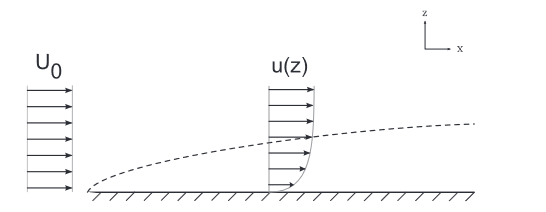
\includegraphics[width=.5\textwidth]{Couchelimitesvisqueuse.png}
  \caption{Couche limite visqueuse au voisinage d'une plaque}
\end{figure}
L'écoulement est stationnaire, incompressible et on suppose qu'il n'existe pas de gradient de pression
horizontal. Appelons respectivement $U$ l'ordre de grandeur de la vitesse $u$, $R$ l'echelle de longueur dans la direction $r$ et $l_v$ celle suivant $z$. On suppose $l_v\ll R$. À l'ordre dominant, l'équation de Navier-Stokes suivant la direction $r$:

\begin{equation}
  \begin{array}{cc}
    \rho v_r \dfrac{\partial v_r}{\partial r}=\eta\dfrac{\partial^2 v_r}{\partial z^2} & \Rightarrow \rho\dfrac{U^2}{R}\sim \eta \dfrac{U}{l_v^2}
  \end{array}
\end{equation}
\begin{figure}[ht]
  \centering
  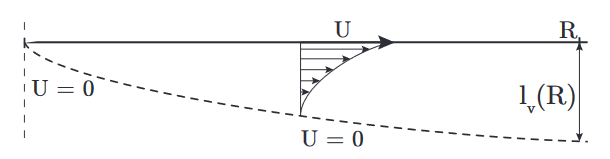
\includegraphics[width=.5\textwidth]{Couchelimitesvisqueuse_marangoni.png}
  \caption{Couche limite visqueuse dans notre système}
\end{figure}

\begin{Programme}{couche limite visqueuse}
  \begin{equation}
    l_v \sim \sqrt{\dfrac{\eta R}{\rho U}}\sim\dfrac{R}{\sqrt{Re}}
  \end{equation}
En dehors de cette couche limite la vitesse est nulle. $v_r$ varie de $U$ à 0 entre $z=0$ et $z= l_v$. Si $Re\gg 1$ $l_v\ll R$.
\end{Programme}

\subsection{Couche limite massique}
De la même manière que la couche limite visqueuse représente l'entraînement visqueux du fluide sur une
certaine  ́epaisseur, un  ́ecoulement arrivant sur un réservoir de matière va entraîner des molécules de ce réservoir sur une  ́epaisseur caratéristique appelée couche limite massique.

\begin{figure}[ht]
  \centering
  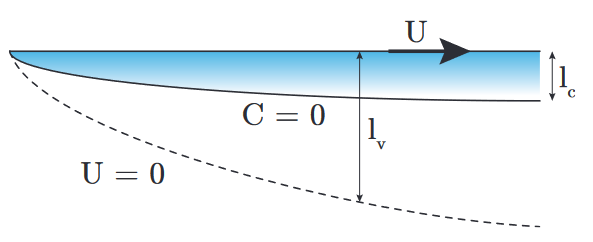
\includegraphics[width=.5\textwidth]{Couchelimitesmassique_marangoni.png}
  \caption{Forme de la couche limite massique}
\end{figure}

Les notations et hypothèses sont les mêmes que pour la couche limite visqueuse, mais cette fois-ci nous appellerons $l_c$ l'échelle de longueur suivant $z$. On suppose $l_c\ll R$, mais  ́egalement $l_c \ll l_v$, ce qui va nous permettre de supposer la vitesse constante et uniforme dans la couche limite massique. À l'ordre dominant, l'équation de convection-diffusion (8) nous donne :

\begin{equation}
  \begin{array}{cc}
  v_r\dfrac{\partial c}{\partial r}=D\dfrac{\partial^2 c}{\partial z^2} & \Rightarrow \dfrac{Uc}{R}\sim \dfrac{Dc}{l_c^2}
  \end{array}
\end{equation}

\begin{Programme}{Couche limite massique}
\begin{equation}
  l_c\sim\sqrt{\dfrac{DR}{U}}=\dfrac{l_v}{\sqrt{Sc}}
\end{equation}
avec $Sc=\dfrac{\eta}{D\rho}$ le nombre de Schmidt qui compare la diffusion de matière aux effets visqueux. Lorsque les effets convectifs dominent $Sc\gg 1$ et $l_c\ll l_v$.  En dehors de cette couche limite, la concentration en surfactants est nulle.
\end{Programme}

\subsection{Continuité de la contrainte tangentielle}

Pour  ́etablir l'équilibre des forces sur le petit morceau d'interface soumi à l'effet Marangoni, un  ́ecoulement est créé dans les 2 fluides environnants et les forces visqueuses qui en découlent viennent assurer l'equilibre. Considérons l'élément d'interface de la figure suivante.

\begin{figure}[ht]
  \centering
  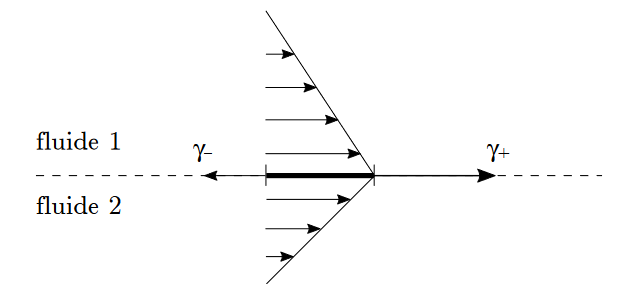
\includegraphics[width=.5\textwidth]{ecoulementinterface.png}
  \caption{Forces agissant sur un morceau d'interface}
\end{figure}

Si on ne considère auxun écoulement perpendiculaire à l'interface entre les deux fluides. Cet élément d'niterface doit être à l'équilibre, on a donc :

\begin{equation}
-\eta_2Ldr\dfrac{\partial v_{r2}}{\partial z}+\eta_1Ldr\dfrac{\partial v_{r1}}{\partial z}+\left(\gamma(r+dr)-\gamma(r)\right)L=0
\end{equation}

Dans le cas où le fluide 1 est de l'air et le fluide 2 de l'eau, on a $\eta_2\frac{\partial v_2}{\partial z}/\eta_1\frac{\partial v_1}{\partial z}\sim \eta_2\frac{\partial v_2}{l_{v2}}/\eta_1\frac{\partial v_1}{l_{v1}}\sim \sqrt{\frac{\eta_2\rho_2}{\eta_1\rho_1}}\sim 10^{-3}$. On pourra donc négliger la contrainte visqueuse due à l'air et on trouve la forme simplifiée: 

\begin{equation}
  \eta\dfrac{\partial v}{\partial z} = \dfrac{\partial \gamma}{\partial r}
\end{equation}

Où $\eta$ et $v$ représentent respectivement la viscosité de l'eau et la vitesse dans l'eau. En loi d'échelle, cette équation donne: 

\begin{Programme}{}
  \begin{equation}
    \begin{array}{cc}
    \eta\dfrac{U}{l_v}\sim\dfrac{\Delta\gamma}{R} & \Rightarrow \sqrt{\eta\rho RU^3}\sim \Delta\gamma
    \end{array}
  \end{equation}
\end{Programme}


\subsection{Conservation de la masse}

Les deux inconnues sont $R$ et $U$ et nous avons qu'une équation (équation 16). On peut fermer le problème en considérant la conservation de la masse de tensioactifs. Les surfactants déposés à la surface ne sont plus à l'interface en dehors de la tâche. En effet, dans le cas contraire, un gradient de tension superficielle subsisterait et ils continueraient à s'étaler par effet Marangoni. Il y a donc égalité des débits de dépôt et de diffusion des tensioactifs vers le volume. L'écoulement de Marangoni correspond à une surface d'échange des tensioactifs entre l'interface et le volume. Par un bilan sur un volume de contrôle d'extension latérale $R$ et d'extension verticale inférieur à $l_c$, la conservation du débit s'exprime: 

\[Q=AD\dfrac{\partial c}{\partial z}\]

Où $A$ est l'aire de l'écoulement de Marangoni. Cette relation donne en loi d'échelle: 
\begin{equation}
  \begin{array}{cc}
  Q\sim AD\dfrac{c^*}{l_c} & \Rightarrow Q\sim Ac^*\sqrt{\dfrac{DU}{R}}
  \end{array}
\end{equation}

\subsection{Lois d'échelles} 

On se retrouve donc avec un système à deux équations et 2 inconnues ($R$ et $U$). Le problème est fermé et nous en déduire les lois d'échelles correspondantes. En configuration axisymétrique la surface d'échange s'exprime $A\sim R^2$, et on trouve: 

\begin{equation}
  \left\{\begin{array}{cc}
    \Delta \gamma & \sim \sqrt{\eta\rho R U^3}\\
    Q &\sim c^*\sqrt{R^3DU}
  \end{array}\right.
\end{equation}

En combinant ces deux équations on peut exprimer la vitesse et la taille de l'écoulement tel que : 
\begin{equation}
  \begin{array}{cc}

  R_{\rm max}^{a} \propto \left(\frac{Q}{c^{*}}\right)^{3/4}\left(\dfrac{\eta\rho}{\Delta\gamma^2 D^3}\right)^{1/8}, & V_{\rm max}^{a}\propto\left(\frac{c^{*}\Delta\gamma^3}{Q}\right)^{1/4}\left(\dfrac{D}{(\eta\rho)^3}\right)^{1/8}.\label{eq:rmarangoni}
      
\end{array}
\end{equation}
 
On peut parvenir à ce résultat en dérivant des équations du mouvement mais c'est long.

\section{Enroulement du tourbillon}

On peut décrire la croissance du tourbillon sous l'écoulement de Marangoni tant qu'il n'intéragit pas avec le fond de la cuve. On considère un écoulement dans une couche d'eau d'épaisseur $h$, de masse volumique $\rho=10^3~\rm kg\cdot m^{-3}$ et de viscosité dynamique $\eta=1\cdot 10^{-3}~\rm Pa\cdot s$. L'écoulement de Marangoni cisaille la surface du liquide avec une vitesse $v_M$ dont la quantité de mouvement diffuse sur une épaisseur $\delta$, la couche limite de vorticité. Par conservation du moment angulaire, lorsque l'écoulement de Marangoni ne transporte plus la couche limite, le fluide se met à tourner sur lui-même et produit un tourbillon. Cet enroulement est toujours en contact avec la couche limite qui l'approvisionne en masse de liquide. Le vortex est caractérisé par son rayon $r$ et sa fréquence angulaire $\omega$. Afin de prédire la croissance de l'enroulement nosu écrivons la conservation de la masse, on néglige la dissipation visqueuse.
\begin{figure}[ht]
  \centering
  %\resizebox{.7\textwidth}{!}{\input{SchemaEnroulement.pdf_tex}}
  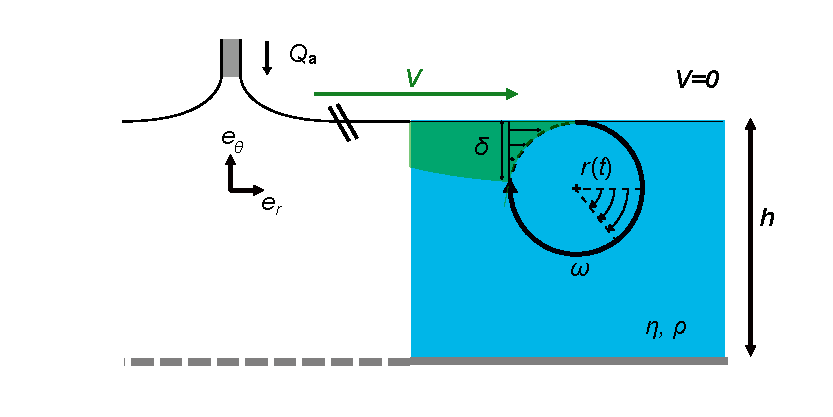
\includegraphics[width=.7\textwidth]{Schema_enroulement_v2.pdf}
  \caption{Schéma du problème}
\end{figure}

On suppose que la couche limite $\delta$ arrivant sur le vortex est complètement absorbée par ce-dernier et qu'il n'y a pas de liquide sortant de l'enroulement. Il en résulte une accumulation de liquide qui n'est possible que s'il y a ybe recirculation de liquide ayant lieu entre le fond du bassun et le liquide. Pour réaliser les calculs on considère une section de l'enroulement, les équations que nous allons écrire sont définies sur une surface coupant le vortex.\medskip

La masse surfacique du vortex s'écrit $m=\pi r^2 \rho$. La variation de la masse du vortex avec le temps provient du flux de liquide advecté par l'écoulement surfacique à travers la couche limite $\delta$.  Le flux de masse entrant dans le vortex s'écrit tel que : $j_m=\rho v\delta$. Et la conservation de la masse traduit la variation de la masse au cours du temps $\dot{m}$ en fonction du flux entrant dans le vortex $j_m$ et du flux sortant qui est supposé nul, d'après nos observations expérimentales. On a alors la relaiton : 

\begin{equation}
  \begin{array}{cc}
    \dot{m} = j_m & \Rightarrow 2r\dot{r}=v\delta
  \end{array}
\end{equation}

Après intégration, on obitent : 

\begin{equation}
  r^2(t)=\dfrac{1}{2\pi}\delta vt+C
\end{equation}
La constante d'intégration C correspond à la valeur initiale du rayon du tourbillon. Le rayon initial doit être de l'ordre de l'épaisseur de la couche limite. On suppose donc que : $r(t = 0 s) = \delta$. Ce qui nous
amène à l'équation décrivant la croissance du rayon du vortex : 

\begin{equation}
  r(t)
=\delta\sqrt{1+\dfrac{vt}{2\pi\delta}}\end{equation}

\section{Modélisation de la propulsion des bateaux de Marangoni}

Dans cette section nous proposons un modèle mathématique pour décrire l'evolution de la vitesse en fonction des paramètres physico-chimiques qui sont: la concentration et la CMC du tensioactif. D'après nos résultats expérimentaux, les bateaux de Marangoni se déplacent spontanément sur la surface de l'eau. Dès que le bateau touche la surface, les tensioactifs s'étalent à l'arrière du bateau. Par conséquent, autour du bateau les tensioactifs sont plus concentrés à l'arrière qu'à l'avant, ce qui génère une différence de tension de surface le propulsant en avant. Tout d'abord, pour décrire le déplacement du bateau nous écrivons l'équation de Newton, puis les équations d'état permettant de relier la variation de la tension de surface à la concentration. Ces équations nous permettront de faire le lien entre la propulsion du bateau et les effets physico-chimiques et thermodynamiques.



\subsection{Bilan des forces}
Le système étudié est celui du bateau se déplaçant dans le plan de la surface de l'eau. Le schéma ci-contre illustre le système étudié (voir figure ci-contre). La cuve sur lequel le bateau se déplace se trouve dans le référentiel du laboratoire lié à la Terre et supposé galiléen. Le principe fondamental de la dynamique s'écrit:

\begin{equation}
  m\frac{d\vv{v}}{dt} = \sum_i{\vv{F_{\rm i}}}
  \label{eqn:Newton}
\end{equation}

\begin{figure}[ht]
  \centering
  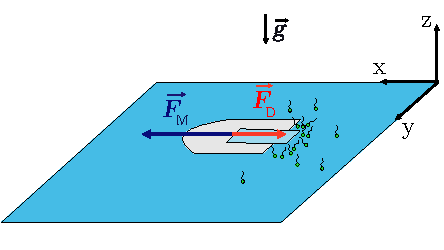
\includegraphics[width=.5\textwidth]{SchemaModeleBateau.pdf}
  \caption{Schéma de la modélisation du bateau de Marangoni}
  \label{fig:ModelSketchBateauMarangoni}
\end{figure}


Les forces perpendiculaires à la surface appliquées au bateau sont: le poids du bateau $\vv{P}=m\vv{g}$ et la force d'Archimède $\vv{P_{\rm A}} = -\rho_{\rm eau} V \vv{g}$. Avec $m=52.2~\rm mg$ la masse du bateau chargé de solution de tensioactif, $\|\vv{g}\| = 9.81~\rm m^2\cdot s^{-1}$ l'accélération de la pesanteur, $\rho_{\rm eau}=1000~\rm kg\cdot m^{-3}$ la masse volumique de l'eau, et $V$ le volume déplacé par le bateau. Le bateau ne se déplace que dans le plan de la surface de l'eau, donc suivant l'axe vertical porté par $\vv{e_{\rm z}}$ la somme des forces est à l'équilibre: 

\begin{equation}
  \rho_{eau} V g = mg \label{eq:SommeDesForcesVerticales}.
\end{equation}

En supposant que le volume de liquide déplacé correspond au volume du bateau immergé $V=L\times W \times \zeta$, nous pouvons calculer de combien le bateau déforme la surface de l'eau. L'équation 25 devient:

\begin{equation}
  \zeta = \frac{m}{\rho_{\rm eau} L W}
\end{equation}
Le bateau déforme la surface et s'enfonce de $z=100~\rm \upmu m$ ce qui est de l'ordre de l'épaisseur de la feuille transparente qui a permis de fabriquer le flotteur. Dans le plan de la surface de l'eau, les forces qui s'appliquent sur le bateau sont la force de propulsion liée à l'effet Marangoni notée $\vv{F_{\rm M}}$ et la force de frottement $\vv{F_{\rm D}}$ opposée au mouvement du bateau.
\subsubsection{La force de frottement}
La force de frottement fluide s'écrit différemment en fonction de la géométrie de l'objet placé dans l'écoulement et suivant la vitesse de l'écoulement. Pour un objet plat, nous pouvons déterminer la force de frottement à partir de la structure de l'écoulement qui a lieu près d'une surface plane.\bigskip

Pour cette démonstration nous nous plaçons dans le référentiel du bateau. Le bateau est donc immobile, et nous considérons l'écoulement qui a lieu autour de lui, en particulier sous la surface. Nous supposons que l'écoulement autour du bateau de Marangoni, est laminaire et uniforme de vitesse $U$ arrivant parallèlement à la plaque qui est le flotteur du bateau. L'écoulement est laminaire mais à grand nombre de Reynolds, car d'après nos mesures expérimentales $R_e$ est compris entre $2582$ et $6951$. Les gradients de vitesse et de vorticité sont concentrés près de la paroi et s'atténuent dans le temps. La distribution de la vorticité le long de la paroi s'élargit par diffusion visqueuse sur une distance $\delta(x)\approx \sqrt{\nu x/U}$, avec $\nu$ la viscosité cinématique du fluide et $x$ la position par rapport à l'arête de la plaque. $\delta$ représente l'épaisseur de la \textbf{couche limite} sur laquelle a lieu la transition entre l'écoulement de fluide loin du flotteur et près de celui-ci. L'écoulement au voisinage de la plaque est contrôlé par la viscosité qui impose une vitesse nulle à la paroi, il vient alors:

\begin{equation}
  \frac{\delta(x_0)}{x_0} \approx \sqrt{\frac{\nu}{Ux_0}}\approx \frac{1}{\sqrt{Re_{x_0}}} \ll 1\label{eq:couchelimitebateau}.
\end{equation}

$Re_{x_0}$ est le nombre de Reynolds local obtenu en prenant la distance $x_0$ à l'arête du flotteur comme échelle de longueur locale. Pour simplifier, nous étudions l'écoulement qui a lieu dans le plan ($xOz$) perpendiculaire à la surface de l'eau. Le bateau est en $z=0$. Nous supposons que l'écoulement est parallèle à la surface de l'eau, suivant la direction $Ox$.

\begin{wrapfigure}[13]{r}{.5\textwidth}%[!ht]
  \centering
  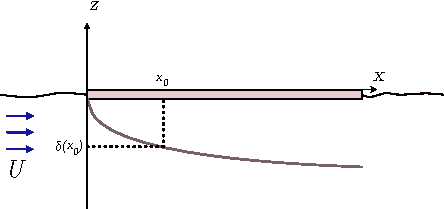
\includegraphics{couchelimitesketch.pdf}
  \caption{Schéma de la couche limite le long du bateau de Marangoni.}
  \label{fig:SketchCouchelimite}
\end{wrapfigure}

Dans la direction parallèle à la surface, la longueur caractéristique correspond à une distance $x_0$ à l'arête du flotteur. Perpendiculairement, la distance caractéristique correspond à l'épaisseur de la couche limite $\delta(x_0) \ll x_0$ défini dans l'équation (27). Pour décrire le mouvement du fluide au voisinage du flotteur, nous écrivons l'équation de la conservation de la masse:

\begin{equation}
  \frac{\partial v_x}{\partial x} + \frac{\partial v_z}{\partial z} = 0 \label{eq:consmass}.
\end{equation}

\noindent Et les équations de Navier-Stokes dans les directions $x$ et $z$ s'écrivent:

\begin{equation}
  \frac{\partial v_x}{\partial t} + v_x\frac{\partial v_x}{\partial x}+v_z\frac{\partial v_x}{\partial z} = -\frac{1}{\rho}\frac{\partial p}{\partial x} + \nu\left(\frac{\partial^2v_x}{\partial x^2}+\frac{\partial^2v_x}{\partial z^2} \right)\label{eq:NSx},
\end{equation}
et:
\begin{equation}
  \frac{\partial v_z}{\partial t} + v_x\frac{\partial v_z}{\partial x}+v_z\frac{\partial v_z}{\partial y} = -\frac{1}{\rho}\frac{\partial p}{\partial z} + \nu\left(\frac{\partial^2v_z}{\partial x^2}+\frac{\partial^2v_z}{\partial y^2} \right) \label{eq:NSz}.
\end{equation}

$v_x$ et $v_z$ sont les composantes de la vitesse du fluide dans les directions $x$ et $z$ au voisinage de la paroi. $p$ est la pression dans le fluide et $\rho$ la masse volumique. À partir des équations 27 et 28 nous pouvons simplifier les équations de Navier Stokes.

\begin{equation}
  v_z\approx v_x\frac{\delta(x_0)}{x_0}\approx v_x. 
\end{equation}

Nous en déduisons que:

\begin{equation}
\frac{\partial^2v_x}{\partial z^2}\approx \frac{v_x}{\delta^2(x_0)} \gg \frac{v_x}{x_0^2} \approx \frac{\partial^2v_x}{\partial x^2},\label{eq:simplx}
\end{equation}

ainsi que :

\begin{equation}
  \frac{\partial^2v_z}{\partial z^2}\approx \frac{v_z}{\delta^2(x_0)} \gg \frac{v_z}{x_0^2} \approx \frac{\partial^2v_z}{\partial x^2}.\label{eq:simplz}
  \end{equation}
  
Par conséquent, nous pouvons réécrire les équations de Navier-Stokes stationnaire ($\partial/\partial t = 0$) sous la forme simplifiée: 

\begin{equation}
  v_x\frac{\partial v_x}{\partial x}+v_z\frac{\partial v_x}{\partial z} = -\frac{1}{\rho}\frac{\partial p}{\partial x} + \nu\frac{\partial^2v_x}{\partial z^2},
\end{equation}
et:
\begin{equation}
 v_x\frac{\partial v_z}{\partial x}+v_z\frac{\partial v_z}{\partial y} = -\frac{1}{\rho}\frac{\partial p}{\partial z} + \nu\frac{\partial^2v_z}{\partial y^2}.
\end{equation}

Les trois termes correspondants à la variation de la vitesse $v_z$ sont négligeables devant les termes de l'équation 35. De même, les fluctuations de pression dans la direction verticale $z$ ont une influence négligeable sur le profil de vitesse par rapport aux variations de pression dans la direction $x$. Par conséquent nous considérons que: $\partial p/\partial z = 0$ et que $p=p(x)$. De plus, en dehors de la couche limite, où les effets de la viscosité sont négligeables, nous pouvons écrire l'équation de Bernoulli le long d'une ligne de courant:

\begin{equation}
  \frac{d p}{dx} +\rho U(x)\frac{dU(x)}{dx}=0
\end{equation}

En remplaçant l'équation 36 dans l'équation 35, on obtient l'équation suivante:

\begin{equation}
  v_x\frac{\partial v_x}{\partial x}+v_z\frac{\partial v_x}{\partial z} = U(x)\frac{dU(x)}{dx} + \nu\frac{\partial^2v_x}{\partial z^2}\label{eq:resNS},
\end{equation}
Maintenant, nous cherchons à déterminer l'équation différentielle vérifiée par le champ de vitesse à l'intérieur de la couche limite. Pour faire cela, nous exprimons la composante de la vitesse $v_x$ qui dépend de $x$ et $z$ en fonction de la variable adimensionnée $\theta$ définie comme $\theta = z/\sqrt{\nu x /U}$  et du module de la vitesse $U$.

\begin{equation}
  v_x(x,z) = Uf(\theta)~~~~~~\text{et}~~~~~~\theta=\frac{z}{\sqrt{\nu x /U}}.
\end{equation}

En remplaçant dans les équations 28 et 38, on obtient l'équation de Blasius:

\begin{equation}
  f''(\theta) = -\frac{1}{2}f'(\theta)\int_0^{\theta}{f(\xi )d\xi}.
\end{equation}

$f(\theta)$ décrit le profil de vitesse $v_x$ au voisinage de la paroi du flotteur comme illustré sur la figure 9.\bigskip 

\begin{wrapfigure}[15]{r}{.45\textwidth}%[!ht]
  \centering
  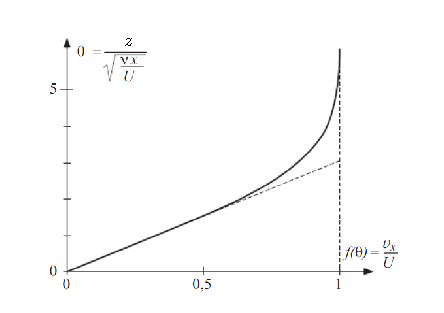
\includegraphics{profilecouchelimite.pdf}
  \caption{Variation de la composante de vitesse en fonction de $\theta$.}
  \label{fig:profilVitesse}
\end{wrapfigure}

À partir de ces résultats nous pouvons déterminer la force de friction de peau entre le liquide et le flotteur du bateau de Marangoni. En effet, la force de frottement par unité de surface à une distance $x$ de l'arête est la composante $\tau_{xz}$ de la contrainte:

\begin{equation}
  \begin{aligned}
    \tau_{xz} &= \eta\left(\frac{\partial v_x}{\partial z}\right)_{z=0}=\eta U f'(0)\frac{\partial \theta}{\partial z}\\
    \tau_{xz} &=\eta U f'(0)\sqrt{\frac{U}{\nu x}}.
  \end{aligned}
\end{equation}

Que nous pouvons réécrire en faisant apparaître, un terme en $U^2$ homogène à une pression:

\begin{equation}
  \tau_{xz} = \rho U^2 f'(0)\sqrt{\frac{\nu}{U x}}.
\end{equation}

Pour obtenir la force totale exercée par le fluide sur la plaque, nous intégrons $\tau_{xz}$ par rapport à $x$ et $y$ sur une des deux faces de la plaque plane de longueur L et de largeur $W$. Il vient alors :

\begin{Programme}{Force de friction sur la paroi du flotteur}
  \begin{equation}
    F_{D} = \rho U^2f'(0)\sqrt{\frac{\nu}{U}}\displaystyle\int_{0}^{w}dy\int_{0}^{L}\frac{dx}{\sqrt{x}}=2\rho w U^2f'(0)\sqrt{\frac{\nu L}{U}} = \beta U^{3/2}.\label{eq:FrottementdePeau}
  \end{equation}

   Pour les calculs de la force, nous considérons que $L$ est la taille du flotteur dans la direction $Ox$ et que la vitesse $U$ est celle du flotteur, enfin $f'(0) \approx 1/3$ d'après Guyon
\end{Programme}


\subsubsection{La force de propulsion}

 Déterminer l'expression de la force de Marangoni est une tâche ardue, car l'effet Marangoni dépend du gradient de concentration des tensioactifs lorsqu'ils s'étalent sur la surface de l'eau. Donc la force capillaire qui dépend de la variation de la tension de surface $\Delta\gamma$ dépend du temps et de l'évolution du profil de concentration $c(r,t)$. Nous proposons un modèle le plus simple possible en exprimant la force de propulsion comme une différence de force capillaire entre l'avant et l'arrière du bateau de la forme:

 \begin{equation}
   F_{\rm M} = \alpha L\Delta\gamma(c(r,t),t). 
 \end{equation}
 
 $\alpha$ est un coefficient géométrique qui dépend de la forme du bateau. $\Delta\gamma$ est la différence de tension de surface entre l'avant et l'arrière du bateau. Nous faisons l'hypothèse que la concentration loin du bateau reste constante pendant toute la traversée du flotteur. De plus, la concentration surfacique de tensioactif au voisinage du bateau à $t=0$ lorsque le bateau touche la surface de l'eau est celle de la solution de tensioactifs dans le réservoir c'est à dire $c(r=0~\rm m,t=0~\rm s) = c_0$.\bigskip

 Ces hypothèses sont fortes, car en pratique la surface de l'eau est rapidement contaminée lors du dépôt du tensioactif donc la concentration loin du bateau devient non-nulle $c_{\infty} \neq 0$. Nous décomposons la variation de la tension de surface en un produit d'une fonction qui dépend de la concentration initiale de tensioactif et d'une fonction qui dépend du temps:

\begin{equation}
  \Delta\gamma(t) = \chi(c_0)\times \xi(t) = \Delta\gamma_0(c_0)\times \xi(t)
\end{equation}

Nous avons vu avec la thermodynamique de l'adsorption des molécules tensioactives qu'il est possible d'obtenir des relations entre la variation de la tension de surface et la concentration en tensioactifs. Nous rappelons l'isotherme de Langmuir : 

\begin{equation}
  \Delta\gamma(c_0) = RT\Gamma_{\infty}\ln{1+K_{\rm L}c_0}
\end{equation}

Cette équation d'état caractérise la variation de la tension de surface lorsqu'un tensioactif est ajouté à l'interface entre deux fluides. Nous choisissons cet isotherme car il prend en compte la saturation de l'interface via la concentration surfacique maximale $\Gamma_{\infty}$. La concentration surfacique maximale est reliée à la concentration en volume et la concentration surfacique à travers l'équation 46 que nous rappelons aussi ci-dessous:

\begin{equation}
  \Gamma(c) = \Gamma_{\infty}\frac{K_{\rm L}c}{1+K_{\rm L}c}.
\end{equation}

R est la constante des gaz parfaits $R = 8.314~\rm J\cdot K^{-1}\cdot mol^{-1}$, $T$ la température en Kelvin (K). $K_{\rm L}$ est la constante de l'équilibre d'adsorption de Langmuir, qui mesure l'efficacité du tensioactif à changer la tension de surface. Pour finir, nous supposons que $\xi(t)$ est de la forme d'une exponentielle décroissante, car les résultats expérimentaux suggèrent que la vitesse du bateau décroît exponentiellement avec le temps, il vient:

\begin{equation}
  F_{\rm M} = \alpha \Delta\gamma_0(c_0){\rm e}^{-\frac{t}{\tau_{\rm M}}}= \alpha LRT\Gamma_{\rm max}\ln(1+K_{\rm L}c_0){\rm e}^{-\frac{t}{\tau_{\rm M}}}.
\end{equation}

$\tau_{\rm M}$ est un temps caractéristique de décroissance de la vitesse du bateau. Pour finir l'équation différentielle générale que nous devons résoudre s'écrit :

\begin{equation}
  m\frac{\mathrm{d}v(t)}{\mathrm{d}t} + \beta v(t)^{3/2} = \alpha L\Delta\gamma_0{\rm e}^{-\frac{t}{\tau_{\rm M}}}.
  \label{eqn:differentielle}
\end{equation}



\subsection{Résolution de l'équation}

\subsubsection{Équation stationnaire}

Dans un premier temps, nous résolvons l'équation stationnaire afin de déterminer la vitesse initiale du bateau $v_0$ lorsque les forces de frottement et de propulsion sont à l'équilibre. L'équation stationnaire est la suivante:

\begin{equation}
  \beta v_0^{3/2} = \alpha L\Delta\gamma(c_0).\label{eq:stationnaire}
\end{equation}


En isolant d'un côté de l'équation la vitesse $v_0$ il vient directement l'expression de la vitesse initiale en fonction de la concentration:

\begin{equation}
  v_0(c_0)=\left(\frac{\alpha RT\Gamma_{\rm max}}{0.664\rho l}\sqrt{\frac{L}{\nu}}\ln(1+K_{\rm L}c_0)\right)^{2/3}.
  \label{eqn:v0}
\end{equation}

Les valeurs de la concentration surfacique maximale $\Gamma_{\infty}$ sont tabulées dans la littérature pour de très nombreux tensioactifs et sont reportées dans le tableau 2 les valeurs présentées dans la littérature. En ce qui concerne $K_{\rm L}$ la constante d'équilibre d'adsorption des tensioactifs de l'isotherme de Langmuir est plus difficile à trouver dans la littérature. Néanmoins, nous avons trouvé la valeur de $K_{\rm L}$ pour trois tensioactifs de la famille des TAB reportés dans la littérature: $\rm C_{14}TAB$, $\rm C_{15}TAB$, $\rm C_{16}TAB$ qui sont indiquées dans le tableau 2  déterminées pour un système à l'\textbf{équilibre}. Nous utiliserons $K_{\rm L}$ et $\alpha$ comme paramètres d'ajustement du modèle afin de le comparer aux expériences.

\begin{table}[ht!]
  \centering
  \begin{tabular}{c|c|c|c}
    \hline \hline
    Tensio-actifs & $\Gamma_{\infty}~\rm (mol\cdot m^{-2})$ & Tensioactifs  &$K_{\rm L }~\rm (m^{3}\cdot mol^{-1})$ \\ \hline \hline
    HTAC, $\rm C_{16}TAC$  & $3.4\cdot 10^{-6}$ &$\rm C_{16}TAB$ & $2.017$ \\ 
    TTAB, $\rm C_{14}TAB$  & $3.3\cdot 10^{-6}$ &$\rm C_{15}TAB$ &$1.5$ \\ 
    DoTAB, $\rm C_{12}TAB$  & $2.9\cdot 10^{-6}$ &$\rm TTAB, C_{14}TAB$ &$1.2$ \\ 
    DeTAB, $\rm C_{10}TAB$  & $2.8\cdot 10^{-6}$ & &\\  \hline
  \end{tabular}
  \caption{Valeurs tabulées dans la littérature pour la concentration surfacique maximale $\Gamma_{\infty}$. Ainsi que pour la constante d'adsorption de Langmuir $K_{L}$.}
  \label{TABLE:Paramv0}
\end{table}

La comparaison entre les résultats expérimentaux et le modèle sont présentés sur la figure 10. En ajustant $\alpha=0.15$ ainsi que $K_{\rm L}$ pour chaque tensioactif, nous obtenons un bon accord entre les courbes et les résultats expérimentaux. L'ajustement de $K_{\rm L}$ nous permet d'obtenir les valeurs indiquées sur le tableau 3 pour les quatre tensioactifs utilisés. Malheureusement, nous ne pouvons pas comparer pour les quatre tensio-actifs à la littérature existante car nous n'avons trouver que des valeurs pour le $C_{14}TAB$.

\begin{figure}[!ht]
  \centering
  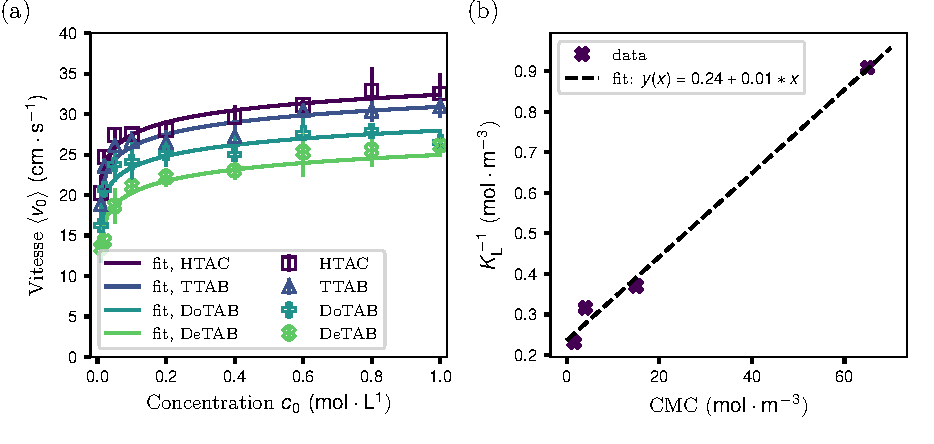
\includegraphics[scale=1]{Vitesse_initiale_versus_concentration_modele.pdf}
  \caption{Comparaison entre les mesures de la vitesse initiale avec le modèle}
  \label{fig:modelev0}
\end{figure}

\begin{table}[ht!]
  \centering
  \begin{tabular}{ccc}
  \hline \hline
  Tensioactif & $K_{\rm L}$ $\rm(m^{3}\cdot mol^{-1})$ ajusté & $K_{\rm L}$ $\rm(m^{3}\cdot mol^{-1})$ littérature \\ \hline \hline
  HTAC, $\rm C_{16}TAC$ & $4.4$ & NA \\
  TTAB, $\rm C_{14}TAB$ & $3.2$ & $1.2$ \\
  DoTAB, $\rm C_{12}TAB$ & $2.7$ & NA \\
  DeTAB, $\rm C_{10}TAB$ & $1.1$ & NA \\ \hline \hline
  \end{tabular}
  \caption{Résultats des ajustements du coefficient d'adsorption de Langmuir $K_{\rm L}$.}
  \label{TABLE:resAjustement}
\end{table}

Nous remarquons qu'il y a un facteur $3$ entre la valeur que nous obtenons et la littérature. Malgré cet écart, l'évolution de $K_{\rm L}$ avec la CMC semble cohérente. En effet pour une concentration donnée, plus la vitesse est grande plus $K_{\rm L}$ est grand. De la même manière, plus la CMC est petite plus $K_{\rm L}$ est grand (voir figure 10\textcolor{blue}{(b)}). Ce graphique traduit l'évolution de l'efficacité des tensio-actifs en fonction de leur nature et de leur affinité avec l'interface. Plus la molécule étudiée présente une valeur élevée de $K_{\rm L}$ plus elle est efficace. C'est effectivement ce que nous observons, Le tensioactif HTAC qui est le plus efficace pour propulser les bateaux obtient la plus grande valeur de $K_{\rm L}$. Et inversement, le DeTAB est le tensioactif qui présente les vitesses les plus faibles et obtient la valeur de $K_{\rm L}$ la plus faible.\bigskip

La réponse linéaire entre $1/K_{\rm L}$ et la CMC rappelle les tendances observées dans la littérature. Cependant Rosen a montré que l'efficacité d'un tensio-actif est dominée par la tête hydrophile du tensioactif, donc tous les $\rm C_{\rm n}TAB$ devraient présenter la même efficacité. Ces résultats sont vrais si la chaîne hydrocarbonée était orientée parfaitement perpendiculairement à l'interface. Cependant, des études plus récentes montrent que les arrangements des tensio-actifs adsorbés sont plus compliqués que cela. La tête hydrophile $\rm Br^{-1}$ peut interagir avec les hydrocarbones ce qui induit des réarrangements de la géométrie de la monocouche de tensioactif à l'interface. Les auteurs montrent que cela joue un rôle significatif sur l'adsorption des tensioactifs. À ces effets, s'ajoutent des phénomènes d'interaction entre ions et contre ions qui peuvent avoir une influence sur l'adsorption. Les résultats montrent que l'efficacité du tensioactif est fortement corrélée à la longueur de la chaîne carbonée: elle augmente non-linéairement avec la longueur de la chaîne. C'est ce que nous observons sur la figure 10\textcolor{blue}{(b)} où nous avons tracé $K_{\rm L}$ en fonction de la CMC sachant que la longueur de la CMC augmente avec le nombre de chaînes carbonées.

\subsubsection{Résolution de l'équation temporelle}

Dans cette section nous proposons de résoudre l'équation temporelle: 

\begin{equation}
  m\frac{\mathrm{d}v(t)}{\mathrm{d}t} + \beta v(t)^{3/2} = \alpha L\Delta\gamma_0{\rm e}^{-\dfrac{t}{\tau_{\rm M}}}.
\end{equation}

Cette équation est difficile à résoudre à la main à cause de la force de frottement qui est proportionnelle à $v^{3/2}$.  Par conséquent, nous cherchons une solution numérique à l'aide de Python et la fonction odeint de la librairie Scipy. Pour résoudre cette équation, nous utilisons les paramètres tabulés dans la littérature pour $\Gamma_{\rm max}$ et calculés pour $K_{\rm L}$. Le paramètre géométrique $\alpha$ est conservé $\alpha= 0.15$. Pour comparer la solution numérique temporelle de la vitesse aux données expérimentales nous ajusteront le paramètre noté $\tau_{\rm M}$ qui correspond au temps caractéristique de décroissance de l'exponentielle. Nous comparons les résultats numériques aux données expérimentales sur la figure 11. Il faut remarquer que le modèle capture assez bien les résultats expérimentaux aux faibles concentrations. Aux grandes concentrations, nous pouvons voir sur la figure 11 que ce n'est pas tout à fait le cas, notamment pour le HTAC et le TTAB qui présentent des paliers pendant la décroissance de la vitesse. Nous n'avons pas d'explication exactes pour ces paliers à l'heure actuelle, nous supposons que c'est un effet de la saturation de l'interface lorsque le réservoir du bateau est très concentré, car ces paliers ne sont pas présents aux concentrations plus faibles. L'ajustement des solutions de l'équation semble mieux marcher pour le DoTAB et le DeTAB. Par conséquent, nous en déduisons la variation de la tension de surface en fonction d'une exponentielle du temps semble une bonne hypothèse pour décrire son évolution au cours du temps.\medskip


\begin{figure}[!ht]
  \centering
  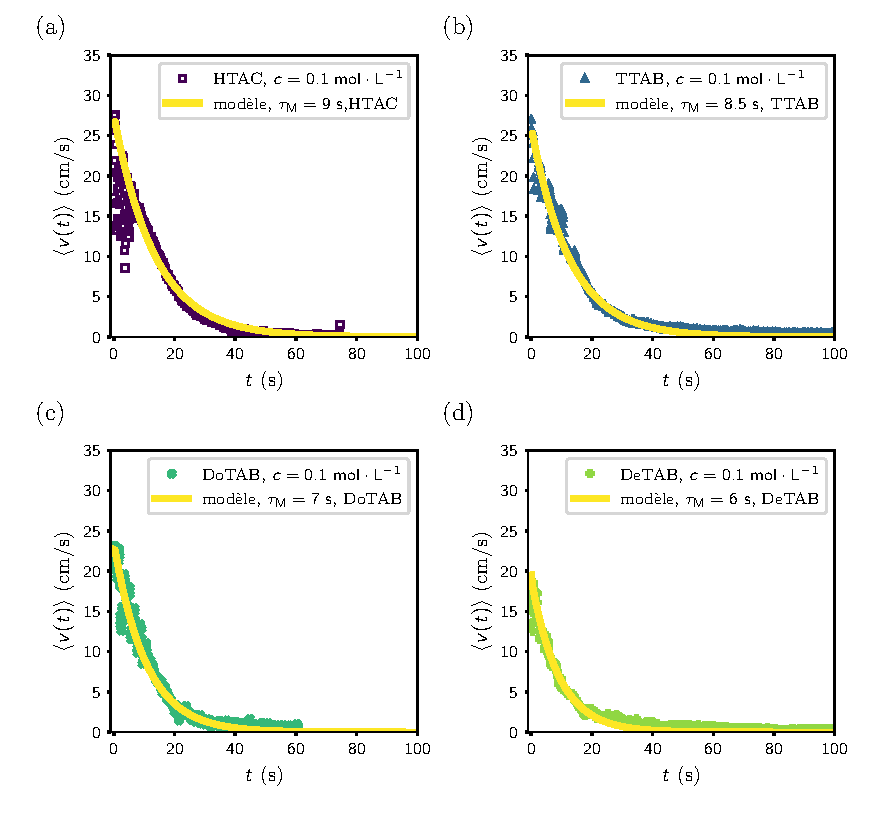
\includegraphics{Deceleration_vitesse_faible_concentration_modele.pdf}
  %\includegraphics[width=.8\textwidth]{./figures/chap5/Deceleration_vitesse_faible_grande_concentration_modele.pdf}
  \caption{Comparaison entre les profils de vitesse expérimentaux et les solutions numériques de l'équation différentielle pour les quatre tensioactifs.}
  \label{fig:decroissancemodele}
\end{figure}

Sur la figure 12 nous avons reporté les valeurs de $\tau_{\rm M}$ qui permettent d'ajuster au mieux les données expérimentales. Le temps caractéristique $\tau_{\rm M}$ augmente avec la concentration $c_0$ initiale de la solution de tensio-actifs. Cela semble cohérent avec nos observations expérimentales puisque plus la solution est concentrée au départ, plus le bateau est capable de maintenir une différence de tension de surface longtemps pour se propulser. De plus, nous pouvons voir que plus la CMC est petite, plus $\tau_{\rm M}$ est grand, ce qui semble cohérent avec la discussion sur l'efficacité du tensioactif. Il faut remarquer que suivant le tensioactif la pente de croissance de $\tau_{\rm M}$ en fonction de la concentration $c$ change. En effet, la pente pour l'HTAC est de l'ordre de $a= 25.6$ tandis que pour le DeTAB $a=6.4$.

  \begin{figure}[!ht]
    \centering
    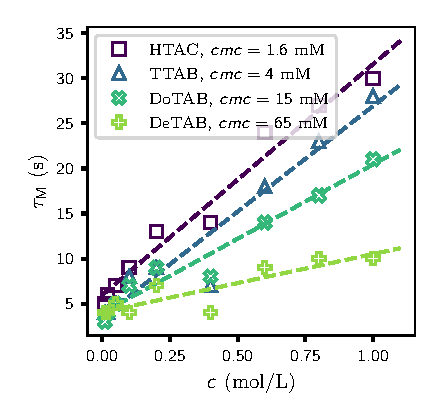
\includegraphics{Temps_caracteristique_versus_concentration.pdf}
    \caption{Mesure du temps caractéristique $\tau_{\rm M}$. Nous avons tracé les régressions linéaires pour chaque tensioactif en pointillés. HTAC: $y(x) = 5.9 + 25.6x$, TTAB:$y(x) = 3.5 + 23.4x$, DoTAB: $y(x) = 3.9 + 16.5x$, DeTAB: $y(x) = 4.0 + 6.4x$. }
    \label{fig:taum}
  \end{figure}
  \noindent \textbf{Ce que nous retenons:}\bigskip

  Bien que le modèle que nous proposons soit très simplifié, nous parvenons à décrire les effets de la thermodynamique sur la propulsion du bateau de Marangoni.\bigskip

  Cependant il nous faut discuter de deux points que nous avons omis dans notre modèle. En effet, nous avons pu remarquer des émissions d'ondes lorsque le bateau se déplace à la surface de l'eau. Or, les ondes sont une source de dissipation d'énergie et donc doivent être prises en compte pour modéliser la propulsion des bateaux. Dans un second temps nous allons discuter de l'influence de l'écoulement de Marangoni sur la propulsion de nos bateaux, car nous avons vu que l'effet de l'écoulement était non-trivial.
\end{document}
% % 
% %
% % FIN DU DOCUMENT
% %
% % 

